
\section{Event-Driven Execution Model} \label{chapter4:event-driven}

The event-driven execution model sequentially processes a queue of asynchronous events by cooperatively scheduling concurrent handlers.
To respond to an event, the associated handler can directly respond to the source of the event.
Or it can request an external resource, and chain another handler to later process the initial event with the resource response, as illustred in figure \ref{fig:cont-chain}.
The developer defines each handler as a continuation and defines their causality using the continuation passing style \cite{Wand1980,Haynes1984}.

\begin{figure}[h!]
  \centering
  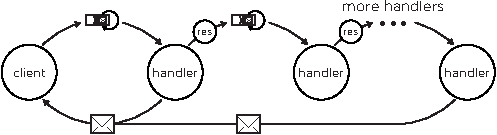
\includegraphics[width=\linewidth]{../resources/cont-chain.pdf}
  \label{fig:cont-chain}
  \caption{Chain of continuations}
\end{figure}

\subsection{Continuation Passing Style} \label{chapter4:event-loop:continuation}

% A callback is a function passed as a parameter to a function call.
% It is invoked by the callee to continue the execution with data not available in the caller context.
% We distinguish three kinds of callbacks.

% \begin{description}
%   \item[Iterators] are functions called for each item in a set, often synchronously.
%   \item[Listeners] are functions called asynchronously for each event in a stream.
%   \item[Continuations] are functions called asynchronously once a result is available.
% \end{description}

% In a synchronous paradigm, the sequentiality of the execution flow is trivial.
% An operation needs to complete before executing the next one.
% In an asynchronous paradigm, parallelism is trivial, but the sequentiality of operations needs to be explicit.

% A continuation is the functional way of defining the causality between two tasks \cite{Wand1980,Haynes1984}.
A continuation is a function passed as an argument to a function call.
% The caller is able to continue the execution while the callee runs in background.
The continuation is invoked later, at the completion of the callee, to continue the execution. % as soon as possible and process the result; hence the name continuation.
When the callee is asynchronous, it allows not to block the caller until its completion.
% It provides a necessary control over the asynchronous execution flow.
% It also brings a control over the data flow which essentially replaces the \texttt{return} statement at the end of a synchronous function.
At its invocation, the continuation retrieves both the caller context, through a closure, and the result.
Listing \ref{lst:continuation} illustrates an example of continuation in \textit{Node.js}.

% The convention on how to hand back the result must be common for both the callee and the continuation.
% For example, in \textit{Node.js}, the signature of a continuation uses the \textit{error-first} convention.
% % \ftnt{https://docs.nodejitsu.com/articles/errors/what-are-the-error-conventions}
% % \ftnt{http://programmers.stackexchange.com/questions/144089/different-callbacks-for-error-or-error-as-first-argument} convention.
% The first argument contains an error or \texttt{null} if no error occurred; then follows the result.
% Listing \ref{lst:continuation} is a pattern of such a continuation.
% However, continuations don't impose any conventions; indeed, other conventions are used in the browser.

\begin{code}[js, %
             caption={Example of a continuation}, %
             label={lst:continuation}] %
callee(input, function continuation(error, result) {
  if (error)
    throw error;
  
  console.log(result);
});
\end{code}

% % The continuation allows to continue the execution sequentially, after the result of \textit{my_fn} is available. 
% % When continuations are defined inside the call, like \textit{continuation}, the sequence of deferred execution results in an intricate imbrication of calls and continuations, like in listing \ref{lst:cbhell}.
% The callback hell occurs when many asynchronous calls are arranged to be executed sequentially.
% Each consecutive operation adds an indentation level, because it is nested inside the continuation of the previous operation.
% % That is when each caller must wait for the result before calling the next function.
% It produces an imbrication of calls and function definitions, as shown in listing \ref{lst:cbhell}.

The continuation passing style lacks the chained composition of multiple asynchronous operations.
% It forces to stack calls of continuations, as illustrated in listing \ref{lst:cbhell}.
Promises improve the composition of continuation.
They allow to arrange such a sequence of asynchronous operations in a chain, similar to a pipeline.

% \begin{code}[js, %
%              caption={Example of a sequence of continuations}, %
%              label={lst:cbhell}] %
% my_fn_1(input, function cont(error, result) {
%   if (!error) {
%     my_fn_2(result, function cont(error, result) {
%       if (!error) {
%         my_fn_3(result, function cont(error, result) {
%           if (!error) {
%             console.log(result);
%           } else {
%             throw error;
%           }
%         });
%       } else {
%         throw error;
%       }
%     });
%   } else {
%     throw error;
%   }
% });
% \end{code}

\subsection{Promise} \label{chapter4:event-loop:promise}

% TODO insert these :
% Promise also provide few methods to enhance the asynchronous control flow tools\footnote{\texttt{all} and \texttt{race}}.
% There is, in Javascript, numerous Promise implementations\footnote{37 different implementations in Javascript \url{https://github.com/promises-aplus/promises-spec/blob/master/implementations.md}}.

% This section is based on the Promises section of the specification in ECMAScript 6 Harmony\ftnt{https://people.mozilla.org/~jorendorff/es6-draft.html\#sec-promise-objects} and the Promises page on the Mozilla Developer Network\ftnt{https://developer.mozilla.org/en/docs/Web/JavaScript/Reference/Global_Objects/Promise}.

% In a synchronous paradigm, the sequentiality of the execution flow is trivial.
In the asynchronous paradigm, the control over the asynchronous execution flow is defined with continuations.
% In the asynchronous paradigm, this control is provided by continuations.
% Promises provide a unified control over the execution flow for both paradigms.
% The ECMAScript 6 specification\ftnt{https://people.mozilla.org/~jorendorff/es6-draft.html\#sec-promise-objects} defines
A Promise is used as a placeholder for the eventual outcome of a deferred (and possibly asynchronous) operation.
% A Promise is an object returned by a function to represent its result
Promises expose a \texttt{then} method which expects a continuation to continue with the result. %; this result being synchronously or asynchronously available.

% However, unlike continuations, the Promises specification imposes a convention on how to handle the result.
% Because it is possibly unavailable synchronously, it still requires a continuation to defer the execution when the result is made available.
% A promise requires two continuations to defer the execution in case of errors.
% These two continuations are passed to the \texttt{then} method of the promise, like illustrated in listing \ref{lst:then}.

% As a result of this difference, Promises and continuations use two different conventions to handle errors and results.
% The two conventions are illustrated in listings \ref{lst:continuation} and \ref{lst:then}.

% \begin{code}[js, %
%              caption={Example of a Promise}, %
%              label={lst:then}] %
% var promise = my_fn_pr(input)

% promise.then(function onSuccess(result) {
%   console.log(result);
% }, function onError(error) {
%   throw error;
% });
% \end{code}

% Continuations lack the chained composition of asynchronous operations.
% Promises are designed to fill the lack of chained composition from continuations.
% They allow to arrange successions of asynchronous operations as a chain of continuations, by opposition to the imbrication of continuations illustrated in listing \ref{lst:cbhell}.
% That is to arrange them, one operation after the other, in the same indentation level.
% The \texttt{then} method synchronously returns a Promise linked with the Promise asynchronously returned by its continuation.
% This link allow to compose chains of asynchronous operations.

The listing \ref{lst:promises-sequence} illustrates this chained composition.
The functions \texttt{callee\_promise\_2} and \texttt{callee\_promise\_3} return promises when they are executed, asynchronously.
Because these promises are not available synchronously, the method \texttt{then} synchronously returns intermediary Promises.
The latter resolve only when the former resolve.
This behavior allows to arrange the continuations as a flat chain of calls, instead of an imbrication of continuations.

\begin{code}[js, %
             caption={Example of a chain of Promises}, %
             label={lst:promises-sequence}] %
callee_promise_1(input)
.then(callee_promise_2, onError)
.then(callee_promise_3, onError)
.then(console.log, onError);

function onError(error) {
  throw error;
}
\end{code}

% The Promises syntax is more concise, and also more readable because it is closer to the familiar synchronous paradigm.
% Indeed, Promises allow to arrange both the synchronous and asynchronous execution flow with the same syntax.
Promises allow to easily arrange the execution flow in parallel or in sequence according to the required causality.
This control over the execution leads to a modification of the control over the data flow.
Programmers are encouraged to arrange the computation as series of coarse-grained steps to carry over inputs.
In this sense, Promises are comparable to an intermediate step toward the pipeline execution model.